\section{Verification-based naming}
\label{sec:verification}


The proposed system can be divided in an enrolment and a search stage. For each person name detected by optical character recognition (OCR), the most likely interval
of speech and face presence are detected and used for enrolment.
%, as depicted in Figure \ref{fig:timeline}. 
Once the detected people are enrolled, speaker and face recognition
are performed for each shot in order to assign labels to that shot. 
A decision fusion strategy is implemented in order to combine the speech and video labels (Fig.~\ref{fig:vbn}). The details of the system
are described below.

\begin{figure}[!htb]
 \centering
 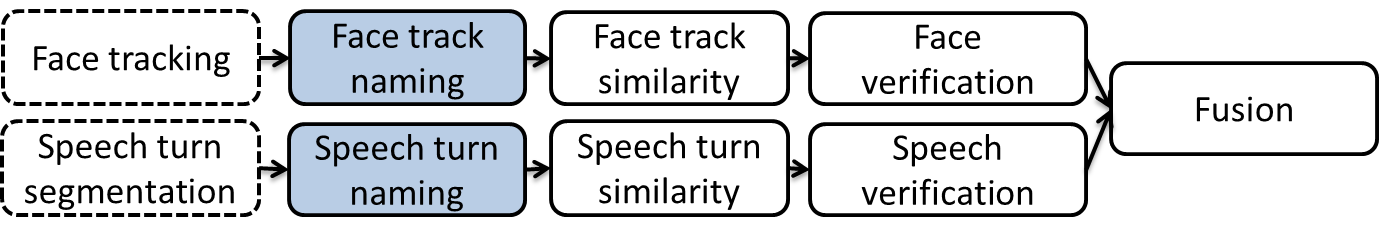
\includegraphics[width=1.\linewidth]{VBN.png}
\vspace*{-5mm}
 \caption{Verification-based naming process. Light blue boxes are when names are combined with face tracks and speech turns to create enrollment models.}
\vspace*{-5mm}
 \label{fig:vbn}
\end{figure}

\subsection{Enrollment}

\subsubsection{GTM-UVigo system}
First, audio and video features were extracted from the recordings. The audio features were 19 MFCCs plus delta, acceleration and energy. For the video features, first
the LIMSI approach was used to detect faces, and then discrete cosine transform (DCT) features were extracted and normalized with Bob toolkit \cite{bob2012}.
%using blocks of size 12
%with 50\% overlap and 45 DCT comonents using the Bob toolkit \cite{bob2012}, preceeded by %geometric normalization and photometric enhancement using the Tan\&Triggs algorithm
%\cite{tan2010}.

For each person name detected by the OCR, the intervals of voice activity detection and appearance of that person were extracted. For the audio, 
the time interval $(t_{\mathrm{start}},t_{\mathrm{end}})$ in which the name of the speaker $spk$ appears is taken as a starting point. A strategy to enlarge this time
 interval in order to obtain more data to enroll the speaker is applied: the boundaries $(t_{\mathrm{start}},t_{\mathrm{end}})$ are iteratively extended $10ms$ to each direction until a change point is detected using the BIC algorithm
for speaker segmentation.
%
% given the time intervals $S_{\mathrm{left}} = (t_{\mathrm{start}}-10,t_{\mathrm{end}})$ and 
% $S_{\mathrm{right}} = (t_{\mathrm{start}},t_{\mathrm{end}}+10)$, a change point is searched within each of these intervals using the Bayesian information criterion algorithm
% (BIC) for speaker segmentation,  having the restriction that the change point has to be in the 
% intervals $(t_{\mathrm{start}}-10,t_{\mathrm{start}})$ and $(t_{\mathrm{end}},t_{\mathrm{end}}+10)$, respectively. If no change point was found within the interval
% $S_{\mathrm{left}}$ then $t_{\mathrm{left}}$ is set to $t_{\mathrm{start}}-10$ and, similarly, if no change point was found within the interval 
% $S_{\mathrm{right}}$ then $t_{\mathrm{right}}$ is set to $t_{\mathrm{end}}+10$. Then, speaker $spk$ is assumed to be speaking in the interval 
% $S_{\mathrm{spk}} = (t_{\mathrm{left}},t_{\mathrm{right}})$. 
% 

For the video, the faces detected by the face tracker in the interval $(t_{\mathrm{start}},t_{\mathrm{end}})$ in 
 which the name of the speaker $spk$ appears were considered.
 %; given that only one face was detected, the whole presence interval of that face is taken but, 
 In case more than one face was detected, the one that appeared in more frames was assigned to the speaker.
 %, assuming that was the dominant face in the given time interval.
 %In case the person appears several times in the OCR output, a segment is computed for each occurrence.
 %
 
 Once the intervals of appearance are defined, an i-vector \cite{dehak10} is extracted for each modality using Kaldi toolkit \cite{kaldi}; in the case of speech, speech activity detection (SAD) was performed beforehand, in order to remove the non-speech intervals. In case several segments were available for a person name, their features were concatenated into a single one.
 %and all the segments  were treated as a single one.

\subsubsection{UPC system}

Using the OCR-NER output, we extracted the \textit{speaker segments/face tracks} temporally overlapping with a written name. These tracks are named 
%with the identity given by the written name 
and will be used to create models for the named person in an unsupervised enrolment step. The models, consisting in a feature vector and a name label, are used to train a verification system.

Speaker information was extracted using an i-vector based speaker tracking system. 
%Assuming that text names are temporarily overlapped with their speaker and face identities, speaker models were created using the data of those text tracks. 
%The baseline speaker diarization was used to select speaker turn segments assigned to OCR names so as to extract the i-vector queries. 
Speaker modelling was implemented using i-vectors \cite{dehak10}. For the feature extraction, 20 MFCCs plus delta and acceleration coefficients were extracted. Using the Alize toolkit\cite{Bonastre1}, a total variability matrix has been trained per show. Therefore, a 400 size i-vector has been extracted for the speaker turn of each query. Those queries with a speaker turn duration beyond 3 seconds were discarded.

We extracted the features from the activation of the last fully connected layer of VGG-face~\cite{parkhi15deep} Convolutional Neural Network (CNN) to train a triplet network architecture~\cite{Schroff2015} using the XXXX face database. An autoencoder was used to reduce the dimensionality of the VGG vectors to 1024. The features from each of the detected faces in each track were extracted and then averaged to obtain a single feature vector.

\subsection{Search}

\subsubsection{GTM-UVigo system}

In order to decide which speaker was present in a shot, first speech and face detection were performed. Speech detection was carried out using a logistic regression approach
used to classify a segment as speech or non-speech, discarding the non-speech segments. For the video, the faces detected by the face tracker within the shot were identified, 
and the one that appeared in more frames (if any) was chosen. After that, the same procedure as in the enrolment stage was performed: features were extracted from the shot
and an i-vector was extracted for each modality (in the case of speech, this was preceded by speech activity detection). Once the i-vectors of the shot were obtained,
cosine scoring with the enrolment i-vectors was computed, choosing the person names that achieved the highest score for each modality. The shot was assigned to
a person if 
%the name assigned by the face and speech modalities were equal and the sum of 
the scores were greater than a threshold.

\subsubsection{UPC system}

For the speech modality, target i-vectors have been extracted from $3s$ segments with a $0.5s$ shift. The identification was performed evaluating the cosine distance of the i-vectors with each query i-vector. The query with the lowest distance was assigned to the segment. A global distance threshold was previously trained with the development database to discard assignations with high distances.

For the video modality, using the set of named tracks from the full video corpus, a Gaussian Naive Bayes (GNB) binary classifier model was trained, using the euclidean distance between pairs of samples from the named tracks. Then, for each specific video, each unnamed track was compared with all the named tracks of the video, computing the euclidean distance between the respective feature vectors of the tracks. This value was classified using the GNB to either being a intra-class distance (both tracks belong to the same identity) or an inter-class distance (the tracks are not from the same person). The probability of the distance being intra-class was used as the confidence score. The unnamed track was assigned the identity of the most similar named track. A threshold on the confidence score (0.75) was used to discard tracks not corresponding to any named track.

\endinput
